\subsection{供給系}
本供給系は植松電機殿の設備を使用した。
供給系系統図を図\ref{fig:LOXLine}に示す。

%\begin{figure}[htbp]
%\begin{tabular}{cc}
%\begin{minipage}{.5\textwidth}
%\begin{center}
%\centering
%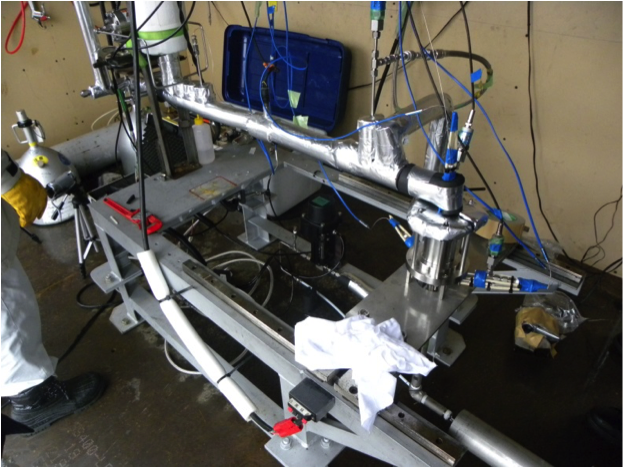
\includegraphics[width=7cm]{\FigAddTwo/LOXLinePho.png}
%\caption{LOXタンク外観}
%\label{fig:LOXTankPho}
%\end{center}
%\end{minipage}
%\begin{minipage}{.5\textwidth}
%\begin{center}
%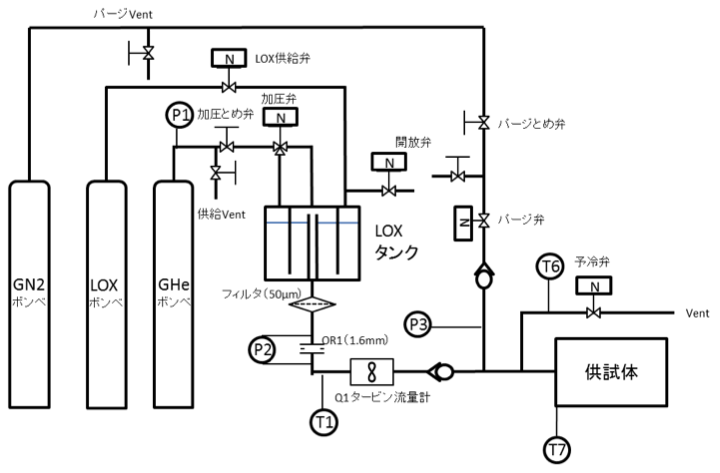
\includegraphics[width=7cm]{\FigAddTwo/LOXLine.png}
%\caption{LOX配管図}
%\end{center}
%\end{minipage}
%\end{tabular}
%\end{figure}

%\begin{figure}
%\centering
%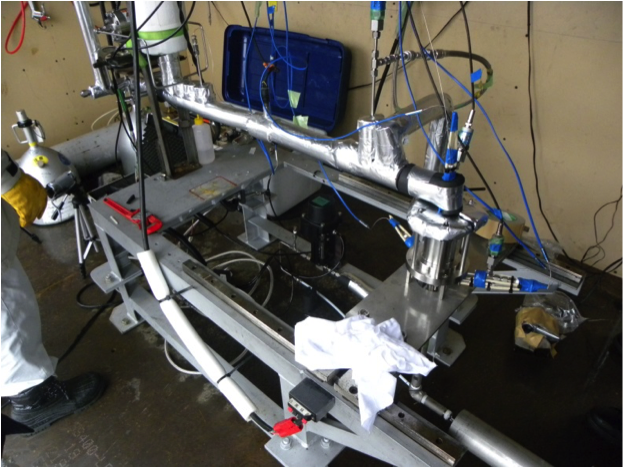
\includegraphics[width=15cm]{\FigAddTwo/LOXLinePho.png}
%\caption{LOXタンク外観}
%\label{fig:LOXTankPho}
%\end{figure}

\begin{figure}
\centering
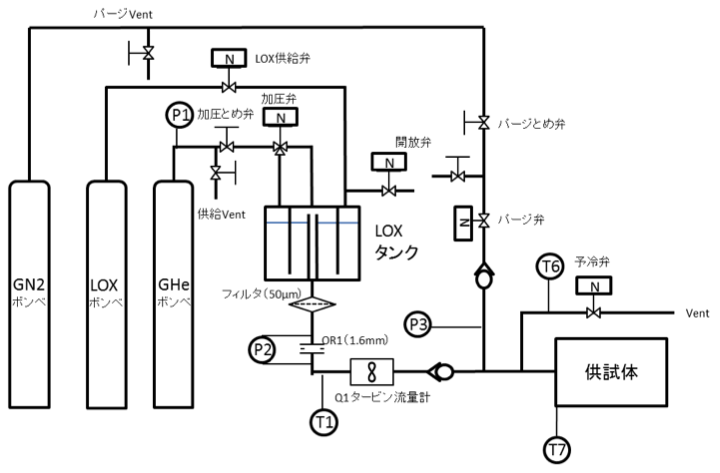
\includegraphics[width=15cm]{\FigAddTwo/LOXLine.png}
\caption{供給系系統図}
\label{fig:LOXLine}
\end{figure}
